\chapter{Árboles Binarios}
Un \textbf{árbol binario} es aquel que cuyos nodos son como máximo de grado 2, es decir, pueden tener 0, 1 ó 2 hijos.

Sabiendo esto vamos a construir nuestros árboles binarios a partir de un árbol completamente vacío, insertando el nodo raíz del mismo y a partir de ahí iremos construyendo el árbol.

Para ello, tenemos que conocer y saber cuales son y que hacen las operaciones que permiten la construcción de árboles binarios, es decir, la \textbf{especificación del TAD árbol binario}.

\section{Especificación del TAD árbol binario}
Sea la especificación de operaciones del TAD Abin (árbol binario):
\subsection*{Constructor del árbol binario}
  \underbar{\textit{Postcondición:}} Crea un árbol completamente vacío.\\
  \verb|  Abin();|

\subsection*{Inserción de nodos}
\begin{itemize}
  \item \underbar{\large\textbf{Inserción del nodo raíz}}:\\
  \underbar{\textit{Precondición:}} Árbol vacío.\\
  \underbar{\textit{Postcondición:}} Inserta el nodo raíz cuyo contenido es `e'.\\
  \verb|  void insertarRaiz(const T& e);|
  \item \underbar{\large\textbf{Inserción de los nodos hijos}}:\\
  \underbar{\textit{Precondición:}} n es un nodo que existe en el árbol y no tiene hijo izquierdo/derecho.\\
  \underbar{\textit{Postcondición:}} Inserta el nodo hijo(izquierdo o derecho) cuyo contenido es `e'.\\
  \verb|  void insertarHijoIzqdo(nodo n, const T& e);|\\
  \verb|  void insertarHijoDrcho(nodo n, const T& e);|
\end{itemize}

\subsection*{Eliminación de nodos}
Para poder eliminar un nodo éste debe de ser un \textbf{nodo hoja}, es decir, no tiene descendientes. Si no hacemos esto, no estaríamos cumpliendo la especificación del TAD.

Además no nos podemos eliminar a nosotros mismo, por tanto, esta operación solamente se podrá realizar a los hijos de nodo, si ese nodo no tiene hijos(es hoja) para eliminarlo tendremos que llamar a su padre y eliminarlo.

\begin{itemize}
  \item \underbar{\large\textbf{Eliminación del nodo raíz}}:\\
  \underbar{\textit{Precondición:}} Árbol no vacío y el nodo raiz es una hoja.\\
  \underbar{\textit{Postcondición:}} Elimina el nodo raíz y deja el árbol vacío.\\
  \verb|  void eliminarRaiz();|

  \item \underbar{\large\textbf{Eliminación de los nodos hijos}}:\\
  \underbar{\textit{Precondición:}} Árbol no vacío y el nodo n no es una hoja.\\
  \underbar{\textit{Postcondición:}} Elimina el nodo hijo izquierdo o derecho del nodo n.\\
  \verb| void eliminarHijoIzqdo(nodo n);|\\
  \verb| void eliminarHijoDrcho(nodo n);|
\end{itemize}

\subsection*{Métodos observadores}
\begin{itemize}
  \item \underbar{\large\textbf{Árbol vacío}}:\\
  \underbar{\textit{Postcondición:}} Devuelve \texttt{TRUE} si el árbol está vacío, si no devuelve \texttt{FALSE}.\\
  \verb|  bool arbolVacio();|
  \item \underbar{\large\textbf{Obtener el elemento de un nodo}}:\\
  \underbar{\textit{Precondición:}} n es un nodo que existe en el árbol. \\
  \underbar{\textit{Postcondición:}} Devuelve el elemento de ese nodo.\\
  \verb|  const T& elemento(nodo n) const;|\\
  \verb|  T& elemento(nodo n);|
  \item \underbar{\large\textbf{Obtener el elemento de la raíz}}:\\
  \underbar{\textit{Postcondición:}} Devuelve el nodo raíz, si el árbol está vacío devuelve \texttt{NODO\_NULO}.\\
  \verb| nodo raiz()const;|
  \item \underbar{\large\textbf{Obtener nodo padre de un nodo cualquiera}}:\\
  \underbar{\textit{Precondición:}} n es un nodo que existe en el árbol.\\
  \underbar{\textit{Postcondición:}} Devuelve el padre del nodo n, si este no tiene devuelve \texttt{NODO\_NULO}.\\
  \verb|  nodo padre(nodo n)const;|
  \item \underbar{\large\textbf{Obtener Hijo Izquierdo de un nodo}}:\\
  \underbar{\textit{Precondición:}} n es un nodo que existe en el árbol.\\
  \underbar{\textit{Postcondición:}} Devuelve el hijo izquierdo del nodo n, si este no tiene devuelve \texttt{NODO\_NULO}.\\
  \verb|  nodo hijoIzqdo(nodo n)const;| 
  \item \underbar{\large\textbf{Obtener Hijo Derecho de un nodo}}:\\
  \underbar{\textit{Precondición:}} n es un nodo que existe en el árbol.\\
  \underbar{\textit{Postcondición:}} Devuelve el hijo derecho del nodo n, si este no tiene devuelve \texttt{NODO\_NULO}.\\
  \verb|  nodo hijoDrcho(nodo n)const;| 
\end{itemize}

\textit{NOTA:} \texttt{NODO\_NULO} no es un elemento, si no que indica la no existencia de un nodo.

\newpage
\section{Implementaciones del TAD árbol binario}
\subsection{Implementación mediante celdas enlazadas}
En esta implementación hacemos uso de memoria dinámica ya que no conocemos el número máximo de nodos que puede contener el árbol.

Vamos a ver dos propuestas de dicha implementación que son correctas pero muy ineficientes:
\begin{figure}[h]
  \begin{minipage}{0.55\textwidth}
    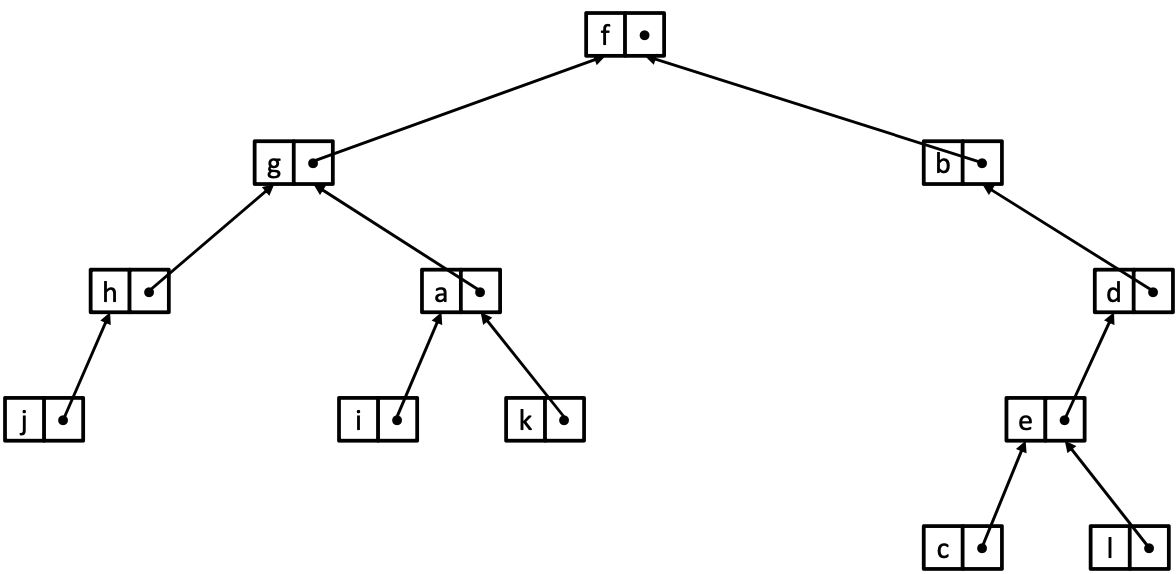
\includegraphics[width=0.8\textwidth]{assets/ICE1.png}
  \end{minipage}
  \hfill
  \begin{minipage}{0.4\textwidth}
    Esta implementación es muy costosa ya que es de orden \(O (n)\) y además al no tener acceso directo al nodo padre ni a los hijos tenemos que acceder desde las hojas, por tanto, al tener que acceder desde las hoja tenemos que recorrer el árbol entero.
  \end{minipage}
\end{figure}

\begin{figure}[h]
  \begin{minipage}{0.55\textwidth}
    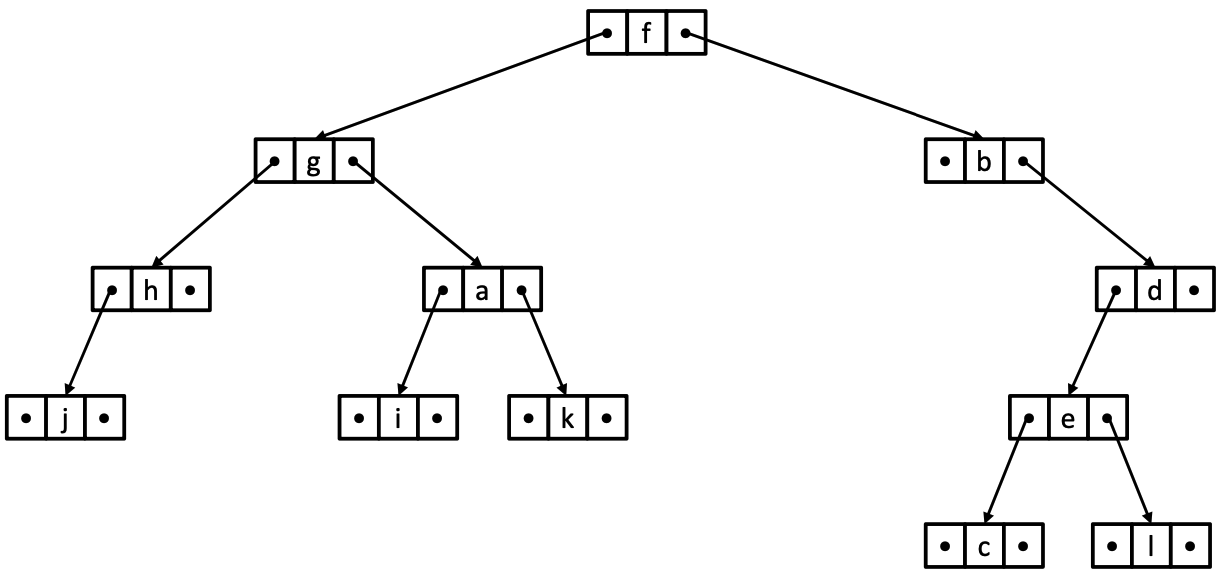
\includegraphics[width=0.8\textwidth]{assets/ICE2.png}
  \end{minipage}
  \hfill
  \begin{minipage}{0.4\textwidth}
    Esta implementación soluciona parcialmente el problema del acceso a los nodos (ya que si podemos acceder a los hijos) pero seguimos sin tener acceso al padre, por lo que su coste sigue siendo \(O (n)\).
  \end{minipage}
\end{figure}

\subsubsection*{Nuestra implementación del TAD árbol binario mediante celdas enlazadas}
\begin{figure}[h]
  \begin{center}
    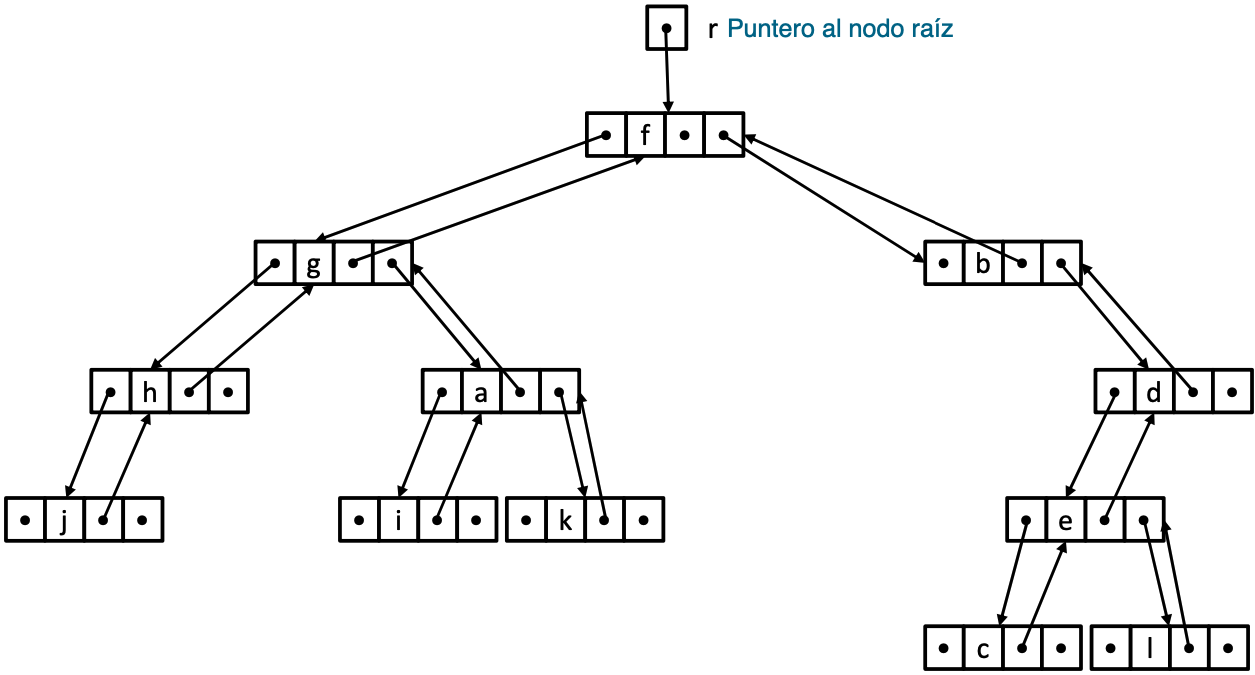
\includegraphics[width=0.8\textwidth]{assets/ICE3.png}
  \end{center}
\end{figure}
Esta será nuestra implementación de dicho TAD, debido a que se corrigen todos los problemas descritos anteriormente, ahora tenemos acceso directo al nodo raíz y podemos acceder a cualquer nodo del árbol.

Finalmente, vemos que gracias a esta implementación todas las operaciones del TAD pasan a ser de orden \(O(1)\).

En memoria se almacenará celdas cuyo contenido son los nodos (padre, hijo izquierdo y derecho) y el elemento del mismo (si ese nodo es nulo, no hay celda), por tanto, en la parte privada del TAD tendremos:
\begin{minted}[breaklines]{C++}
template <typename T> class Abin{
  public:
    //Métodos vistos en la especificación del TAD
  private:
    struct celda{
      T elto; //elemento del nodo
      nodo padre, hizq, hder; //nodos
      celda(const T& e, nodo p = NODO_NULO):elto(e),padre(p),
      hizq(NODO_NULO),hder(NODO_NULO){}
    };
    nodo r; //nodo raíz del árbol.
};
\end{minted}
\subsubsection*{Notas sobre el código de la implementación del TAD}
En la parte pública de la clase encontramos:\\
\verb|  static const nodo NODO_NULO;|, que nos va a permitir indicar explicitamente la no existencia de un nodo.

A la hora de construir un Abin, este se debe de crear vacío, es decir, el nodo raíz es un nodo nulo:\\
\verb|  template <typename T> inline Abin<T>::Abin():r(NODO_NULO){}|

Cuando vayamos a insertar el nodo que será la raíz del árbol solo le pasamos el contenido del mismo, ya que al tener un puntero a la raíz no nos hace falta pasarle el nodo:
\begin{minted}[breaklines]{C++}
template <typename T> inline void Abin<T>::insertarRaiz(const T& e){
  assert(r == NODO_NULO); //Comprobamos la Precondición
  r = new celda(e); //Inserción del nodo raíz.
}
\end{minted}

Si queremos insertar ya sea un nodo hijo izquierdo o derecho, tenemos que pasarle el nodo n (padre de ese nuevo nodo) y el elemento del nodo a insertar.
\begin{minted}[breaklines]{C++}
template <typename T> inline void Abin<T>::insertarHijoIzqdo(nodo n, const T& e){
  //Comprobamos Precondiciones
  assert(n == NODO_NULO); 
  assert (n->hizq ==NODO_NULO);
  n->hizq = new celda(n,e); //Inserción del nodo hijo izquierdo de n.
}
\end{minted}
\textit{NOTA:} Análogamente para la inserción del hijo derecho de un nodo.

Si queremos eliminar un nodo, este debe ser una hoja. Por tanto, primero debemos comprobar si el nodo es una hoja. Si lo es, lo eliminamos dejándolo como un nodo nulo. Esto asegura que el nodo quede en un estado válido y que la dirección de memoria que ocupa la celda se libere correctamente.
\begin{minted}[breaklines]{C++}
template <typename T> inline void Abin<T>::eliminarHijoIzqdo(nodo n){
  //Comprobamos Precondiciones
  assert(n==NODO_NULO);
  assert(n->hizq!=NODO_NULO);//existe hijo izquierdo
  assert(n->hizq->hizq==NODO_NULO && n->hizq->hder==NODO_NULO); //Es Hoja

  //Lo explicado anteriormente
  delete n->hizq; //eliminamos
  n->hizq = NODO_NULO; //lo dejamos en estado válido
}
\end{minted}
\textit{NOTA:} No podemos hacer estos dos últimos paso a la inversa debido a que si lo dejamos como estado válido (nodo nulo), no podremos eliminar el puntero ni la dirección de memoria.
\textit{NOTA:} Análogamente para la eliminación del hijo derecho de un nodo.

Por otro lado, encontramos si queremos eliminar la raíz de un árbol, esta debe de ser una hoja, y por ende al ser eliminado dicho nodo el árbol quedaría vacío.
\begin{minted}[breaklines]{C++}
template <typename T> inline void Abin<T>::eliminarRaiz(){
  //Comprobamos Precondiciones
  assert(r == NODO_NULO);
  assert(r->hizq == NODO_NULO && r->hder == NODO_NULO);
  delete r;
  r = NODO_NULO;
}
\end{minted}

Dentro de la parte privada del TAD encontramos dos métodos:
\begin{itemize}
  \item \verb|DestruirNodos(nodo& n)|; donde dado un nodo n elimina todos los descendientes del mismo, para poder eliminar al mismo. Esto nos simplifica mucho el destructor de la clase ya que al ser un método recursivo se ejecuta tantas veces hasta que llega a la condición de parada `NODO\_NULO'.
  \begin{minted}[breaklines]{C++}
template <typename T> void Abin<T>::destruirNodos(nodo& n){
  if(n!= NODO_NULO){
    destruirNodos(n->hizq);
    destruirNodos(n->hder);
    delete n;
    n=NODO_NULO;
  }//Para cuando n = NODO_NULO
}
  \end{minted}
  \item \verb|Copiar(nodo n)|; dado un nodo n cualquiera realiza una copia de dicho nodo y todos sus descendientes, donde ese nodo n es la raíz del nuevo árbol creado.
  \begin{minted}[breaklines]{C++}
template <typename T> typename Abin<T>::nodo Abin<T>::copiar(nodo n){
  nodo m = NODO_NULO; //creamos un nodo m aux
  if(n!= NODO_NULO){
    m = new celda(n->elto); //copiamos el padre (n).
    m->hizq = copiar(n->hizq); //copiamos subárbol izquierdo recursivamente
    if(m->hizq != NODO_NULO)
      m->hizq->padre = m;
    m->hder = copiar(n->hder); //copiamos subárbol derecho recursivamente
    if(m->hder != NODO_NULO)
      m->hder->pader = m;
  }
  return m;
}
  \end{minted}
\end{itemize}
\subsection{Implementación vectorial del TAD árbol binario}
A diferencia de la implementación mediante celdas enlazadas aquí si conocemos el número máximo de nodos del árbol, además haremos uso de un vector (como bien dice su nombre) de celdas que también almacenará el elemento y los nodos padre, hijo izquierdo y derecho. Véase \textit{Figura 2.1: Representación de la implementación vectorial.}

\begin{figure}[h]
  \begin{center}
    \includegraphics*[width=\textwidth]{assets/IVEC1.png}
  \end{center}
  \caption{Representación de la implementación vectorial.}
\end{figure}

Ahora en la parte privada del TAD encontramos dos variables \texttt{numNodos}(número actual de nodos del árbol) y \texttt{maxNodos}(tamaño del árbol), ahora tenemos que tener en cuenta al primero para poder insertar y eliminar en coste unitario (\(O(1)\)), el segundo nos hará falta para poder crear el árbol ya que en este caso el constructor recibe por parámetro el numero máximo de nodos, es decir, \texttt{maxNodos} → \verb|Abin(size_t maxNodos);|

Para que la eliminación de nodos sea de coste unitario debemos de mover el último nodo insertado a la última posición del vector.

\subsubsection*{Implementación de Inserción y Eliminación de los nodos}
\begin{itemize}
  \item \underbar{\large\textbf{Inserción}}: En la inserción de un nodo tenemos que tener en cuenta el número actual de nodos que hay en el árbol ya que este tiene que ser menor a \texttt{maxNodos}, esto nos ayudará a que la inserción sea de coste unitario, ya que accedemos a la última posición del vector (sin tener que recorrer todo el árbol):
  \begin{minted}[breaklines]{C++}
template <typename T>
inline void Abin<T>::insertarHijoIzqdo(nodo n, const T& e){
  //Precondiciones
  assert(n>=0 && n <numNodos); //nodo valido
  assert(n->hizq == NODO_NULO); //n no tiene hijo izquierdo previo
  assert(numNodos < maxNodos); //árbol no lleno
  //Inserción del nodo
  nodos[numNodos].hizq = numNodos; //el nuevo nodo se inserta al final
  nodos[numNodos].elto = e; //almacenamos el elemento
  nodo[numNodos].hizq = NODO_NULO; //no tiene hijo izquierdo
  nodo[numNodos].hder= NODO_NULO; //no tiene hijo derecho
  numNodos ++; //incrementamos el número de nodos actuales en el vector.
}
  \end{minted}
  \item \underbar{\large\textbf{Eliminación}}: La eliminación de un nodo siempre va a ser de coste unitario, debido a que se elimina el hijo de un nodo n `padre' (el cual tenemos acceso directo).
  \begin{minted}[breaklines]{C++}
template <typename T> inline void Abin<T>::eliminarHijoIzqdo(nodo n){
  nodo hizqdo; //creamos un nodo auxiliar
  //Precondiciones
  assert(n>=0 && n < numNodos);
  hizqdo = nodos[n].hizq; //guardamos el hijo izquierdo del nodo n
  assert(hizqdo != NODO_NULO); //existe hijo izquierdo de n
  assert(nodos[hizqdo].hizq == NODO_NULO &&
    nodos[hizqdo].hder == NODO_NULO); // es Hoja
  
  //Comprobamos si el hijo izquierdo de n no es el último nodo insertado.
  if(hizqdo != numNodos - 1){
    //Movemos el último nodo a la posición del hijo izqdo
    nodos[hizqdo] = nodos[numNodos-1];
    //Actualizamos la posición del hijo en la padre del nodo movido(hizqdo)
    if(nodos[nodos[hizqdo].padre].hizq == numNodos - 1){
      nodos[nodo[hizqdo].padre].hizq = hizqdo;
    }
    else{
      nodos[nodos[hizqdo].padre].hder = hizqdo;
    }
    //Si el movido tiene hijos, solamente cambiamos el padre
    if(nodos[hizqdo].hizq!=NODO_NULO) //Si tiene hijo izquierdo
      nodos[nodo[hizqdo].hizq].padre = hizqdo;
    if(nodos[hizqdo].hder != NODO_ NULO)
      nodos[nodos[hizqdo].hder].padre = hizqdo;
  }
  nodos[n].hizq = NODO_NULO;
  --numNodos;
}
  \end{minted}
\end{itemize}
Es decir, movemos el último nodo insertado a la posición del nodo que vamos a eliminar para que podamos insertar siempre por el final (última posición del vector) haciendo que sea de coste unitario.\\
\textit{NOTA}: Análogamente para el hijo derecho.

\subsection{Implementación mediante vector de posiciones relativas}
En esta implementación no nos hará falta almacenar punteros para poder acceder a los nodos Hijos y padre, es decir, vamos a poder acceder a ellos sin que estén almacenados.

Ahora la variable \texttt{maxNodos} se calculará mediante una fórmula donde estará implicada la altura \(h\) que coindice con el nivel de nodo.\\
Sea la formula: \texttt{maxNodos} = \(\sum_{i=0}^{h} 2^i = 2^{h+1}-1\).

También podemos calcular las posiciones de los nodos:
\begin{itemize}
  \item \texttt{padre(i)} = \((i-1)/2\) (división entera).
  \item \texttt{hizq(i)} = \(2i+1\), los impares son hijos izquierdos.
  \item \texttt{hder(i)} = \(2i+2\), los pares son hijos derechos.
\end{itemize}

Gracias a esto, solamente almacenamos un vector cuyo contenido es el elemento de cada nodo y cada posición del vector corresponde al nodo (calculado mediante las fórmulas anteriores).
Véase (\textit{Figura 2.2: Ejemplo de la representación con un vector de posiciones relativas}).
\\
Para un árbol binario:
\begin{figure}[h]
  \begin{minipage}{0.39\textwidth}
    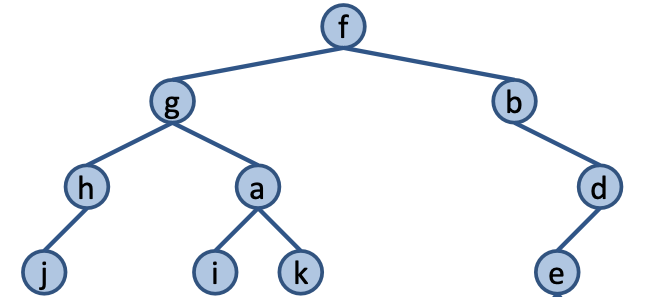
\includegraphics[width=\textwidth]{assets/IVPR.png}
  \end{minipage}
\hfill
\begin{minipage}{0.6\textwidth}
    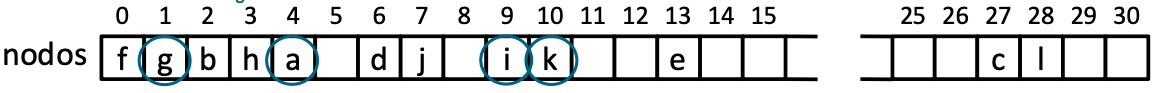
\includegraphics[width=\textwidth]{assets/IVPR2.png}
    Encontramos el vector que contiene los elementos de cada nodo, asi vemos que en la posición 4 (hijo derecho de g) encontramos el elemento `a'.\\
    Ejemplo: \texttt{hder(g)} = \texttt{hder(1)} = \(2*1+2\) = 4.
\end{minipage}
\caption{Ejemplo de la representación con un vector de posiciones relativas}
\end{figure}

Esta implementación tiene una parte mala y es que encontramos un caso muy desfavorable, esto es debido a que el tamaño del vector depende de la altura del árbol, por tanto, si encontramos la ausencia de nodo en un nivel \(n \leq h\) provocará \(2^{h-n+1}-1\) posiciones libres en el vector.

Veámoslo con un ejemplo:
\begin{figure}[h]
  \begin{minipage}{0.39\textwidth}
    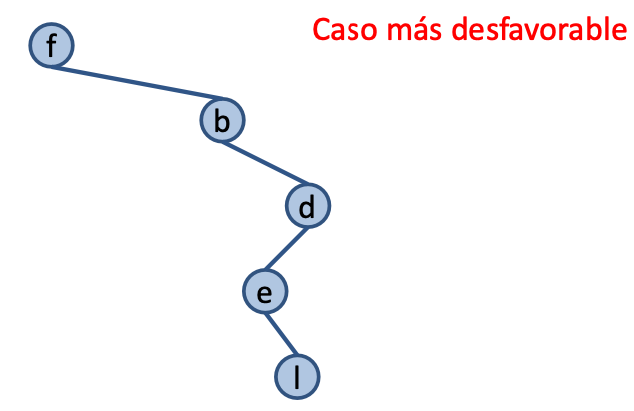
\includegraphics[width=\textwidth]{assets/IVPR3.png}
  \end{minipage}
  \hfill
  \begin{minipage}{0.6\textwidth}
    \includegraphics*[width=\textwidth]{assets/IVPR4.png}
    Si queremos que el nodo con elemento \(l\)(posición 28) tenga tanto hijo izquierdo como derecho, estos quedarán en las posiciones del vector \(2*28+1 = 57\) y \(2*28+2 = 58\) del vector, es decir, duplicamos el tamaño del vector solamente para insertar 2 nuevos nodos, un gasto de memoria excesivo.
  \end{minipage}
\end{figure}
\newpage
Por otro lado, tenemos un caso muy favorable y sucede cuando tenemos el árbol casi completo, es decir, no hay ausencia de nodos por nivel (todos los niveles tienen todos los nodos que les corresponde), lo denominamos como \textbf{árbol completo}.

\begin{figure}[h]
  \begin{minipage}{0.39\textwidth}
    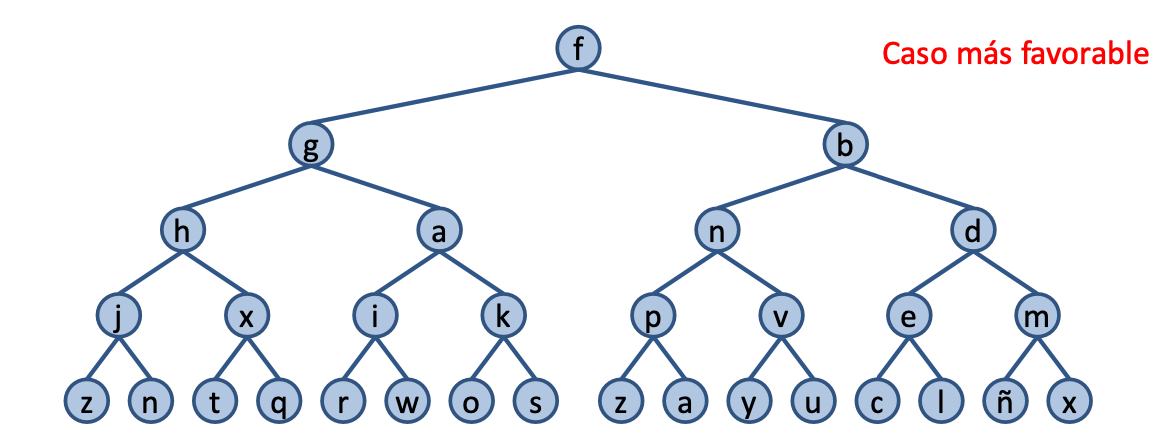
\includegraphics[width=\textwidth]{assets/IVPR5.png}
  \end{minipage}
  \hfill
  \begin{minipage}{0.6\textwidth}
    \includegraphics*[width=\textwidth]{assets/IVPR6.png}
    En esta implementación la eficiencia espacial será mejor cuanto más lleno esté el árbol, es decir, cuanto menos posiciones falten por ser rellenadas en el vector.
  \end{minipage}
\end{figure}

Finalmente, hacemos uso del concepto de \textbf{elemento nulo} \texttt{T ELTO\_NULO}, no es un elemento o contenido del nodo, si no que al igual que NODO\_NULO, indica la no existencia de elemento en el vector, es decir, una \textbf{flag} que nos indica las posiciones libres del vector (\textit{Figura 2.3:Vector nodos con el uso de elemento nulo}).
\begin{figure}[h]
  \begin{center}
    \includegraphics*[width=\textwidth]{assets/IVPR7.png}
  \end{center}
  \caption{Vector nodos con el uso de elemento nulo}
\end{figure}